% ********************************************
%
%   Dear Authors,
% 
%   Please, read the following comments in Preset settings and adjust the settings according to your needs.
%   Please, feel free to add more packages or macros if needed.
%   Details of the pre-defined packages, symbols and macros can be found in the submodule "template". (See PDF files.)
%   If you finished the adjustments, you can remove the comments for a clean document.
% 
%   Any questions or contributions are welcome.
%   Please, contact to the author.
%   Enjoy your writing.
%
%                               Myeongseok Ryu
%  	    				dding_98@gm.gist.ac.kr
%                                  09.Feb.2025
%
% ********************************************

% ********************************************
% Revision History
%   - 01.Jun.2025: Journal template created.
% ********************************************

% ********************************************
% This project is highly ispired by the work of LMRES Lab, Hochschule München.
% Thank you very much my dear friend, Niklas Monzen, for your kind support.
% ********************************************

% ============================================
%         Preset 1. Document Type
% ============================================
\documentclass[lettersize,journal]{IEEEtran}

% ============================================
%         Preset 2. Local Path
% ============================================
% When you create "figures" or "movies" directories in the "src" (source code) directory, the file name including path can be long.
% To avoid this, and to make it easier to adjust, you can define the alias for the path.
% The examples are provided below.

\newcommand*{\FIGURESPATH}{./figures}
% \newcommand*{\SIMFIGURESPATH}{./src/script_simulation/figures}
% \newcommand*{\SLXFIGURESPATH}{./src/simulink_simulation/figures}
% \newcommand*{\MOVIESPATH}{./movies}

% ============================================
%         Preset 3. Pre-defined Settings
% ============================================
% PLEASE DO NOT ADD OR REMOVE PACKAGES IN THE SUBMODULE LOCALLY!
% CONTACT THE AUTHOR FOR ADJUSTMENTS.
%
% The packages are pre-defined in the submodule "Template".
% If you need more packages, please add them after using pre-defined packages.

\def\pub{false} % true for publication, false for draft
\newcommand*{\template}{..} 
% ============================================
%         PATH DEFINITION
% ============================================
\newcommand*{\MACRO}{\template/macros}
\newcommand*{\SYMBOL}{\template/symbols}
\newcommand*{\PACKAGE}{\template/packages}

% ============================================
%         PACKAGES LOAD
% ============================================
% ============================================
%         General Packages
% ============================================
\usepackage{balance}

\usepackage{kotex}      % for Korean
\usepackage{lipsum}     % for dummy text
\usepackage{array}

\usepackage{cite}   % for citation
% \usepackage[
%     backend=biber,
%     % style=authoryear,
%     % doi=false,
%     isbn=false,
%     url=false,
%     minnames=1,
%     maxcitenames=2, maxbibnames=6,
%     % natbib=true,
%     style=ieee,
%     sorting=none,
% ]{biblatex}

\usepackage{amsmath,amsfonts}
\usepackage{amssymb}
\usepackage{soul}

\def\publish{true}
\def\draft{false}
\usepackage{hyperref}
\ifx \pub\publish % Publish
    \hypersetup{
        pdftoolbar=false,        	% show Acrobat’s toolbar?
        pdfmenubar=false,        	% show Acrobat’s menu?
        pdffitwindow=false,     	% window fit to page when opened
        pdfstartview={FitH},    	% fits the width of the page to the window
        pdftitle={},    	% title
        pdfauthor={},     	% author
        %     pdfsubject={},   	% subject of the document
        %     pdfcreator={},   	% creator of the document
        %     pdfproducer={}, 	% producer of the document
        %     pdfkeywords={keyword1, key2, key3}, % list of keywords
        %     pdfnewwindow=true,      	% links in new PDF window
        colorlinks=true,       	% false: boxed links; true: colored links
        linkcolor=black,          	% color of internal links (change box color with linkbordercolor)
        citecolor=black,       	% color of links to bibliography
        filecolor=black,      	% color of file links
        urlcolor=black		% color of external links
    }
\else % Draft
    \hypersetup{
        pdftoolbar=false,        	% show Acrobat’s toolbar?
        pdfmenubar=false,        	% show Acrobat’s menu?
        pdffitwindow=false,     	% window fit to page when opened
        pdfstartview={FitH},    	% fits the width of the page to the window
        pdftitle={},    	% title
        pdfauthor={},     	% author
        %     pdfsubject={},   	% subject of the document
        %     pdfcreator={},   	% creator of the document
        %     pdfproducer={}, 	% producer of the document
        %     pdfkeywords={keyword1, key2, key3}, % list of keywords
        %     pdfnewwindow=true,      	% links in new PDF window
        colorlinks=true,       	% false: boxed links; true: colored links
        linkcolor=blue,          	% color of internal links (change box color with linkbordercolor)
        citecolor=blue,       	% color of links to bibliography
        filecolor=blue,      	% color of file links
        urlcolor=blue		% color of external links
    }
\fi


% \usepackage{cleveref}
% \let\etoolboxforlistloop\forlistloop % save the good meaning of \forlistloop
% \usepackage{autonum}
% \let\forlistloop\etoolboxforlistloop % restore the good meaning of \forlistloop

\usepackage{algorithm}
\usepackage{algorithmic}

\usepackage{epsfig}
\usepackage[dvipsnames]{xcolor}

% MY PACKAGES ===================================

\usepackage{svg}
\usepackage{subfig}

\usepackage{textcomp}
\usepackage{stfloats}
\usepackage{url}
\usepackage{verbatim}
\usepackage{graphicx}
\usepackage{multirow}
\usepackage{multicol}

\let\proof\relax
\let\endproof\relax
\usepackage{amsthm}
\usepackage{lipsum}
\usepackage{tikz}


% ============================================
%         MACROS Packages
% ============================================

\newcommand{\KHCH}[1]{{\color{RoyalPurple} [KH: #1]}} % Kyunghwan's
\newcommand{\MSRY}[1]{{\color{Peach} [MS: #1]}} % Myeongseok's 
\newcommand{\SHJH}[1]{{\color{green} [SH: #1]}} % Seunghun's 
\newcommand{\DHHO}[1]{{\color{magenta} [DH: #1]}} % Donghwa's 

\newcommand{\etal}{\textit{et~al.\ }}
\newcommand\eg{\textrm{e.g.,\ }}
\newcommand\ie{\textrm{i.e.,\ }}

\newcommand{\colorLine}[2]{[\tikz[baseline=(current bounding box.base)]{\draw[color=#1,
#2,line width=2pt] (0,3pt) -- (1.5em,3pt);}]}


\newcommand\R{\mathbb{R}}

\newcommand*{\mv}[1]{\boldsymbol{#1}} % my vector
\newcommand*{\mm}[1]{\boldsymbol{#1}} % my matrix
\newcommand*{\norm}[1]{\lVert #1 \rVert} % euclidean norm

% ============================================
%         FRACTIONS
% ============================================
\newcommand\der{\mathrm d}
\newcommand*{\ddt}{
    \frac{\der}{\der t}
}
\newcommand*{\ddtt}{
    \tfrac{\der}{\der t}
}
\newcommand*{\ddttddtt}{
    \tfrac{\der^2}{\der t^2}
}
\newcommand*{\ddfrac}[2]{
    \frac{\der {#1}}{\der {#2}}
}
\newcommand*{\ddtfrac}[2]{
    \tfrac{\der {#1}}{\der {#2}}
}
\newcommand*{\ppfrac}[2]{
    \frac{\partial {#1}}{\partial {#2}}
}
\newcommand*{\pptfrac}[2]{
    \tfrac{\partial {#1}}{\partial {#2}}
}

% ============================================
%         OPERATORS
% ============================================
\DeclareMathOperator{\myvec}{vec}       % vectorization
\DeclareMathOperator{\myproj}{{Proj}}   % projection
\DeclareMathOperator{\mysat}{sat}       % saturation
\DeclareMathOperator{\myrow}{row}       % row of a matrix
\DeclareMathOperator{\mycol}{Col}       % column of a matrix
\DeclareMathOperator{\mysym}{sym}       % symmetric part of a matrix
\DeclareMathOperator{\mydiag}{diag}     % diagonal matrix
\DeclareMathOperator{\mysign}{sign}     % sign function
\DeclareMathOperator{\mypoly}{Poly}     % polynomial

  

% ============================================
%         SYMBOLS Packages
% ============================================
% ============================================
%         NEURAL NETWORKS
% ============================================
\newcommand*{\NN}{\mv{\Phi}}
\newcommand*{\act}{\mv{\phi}}
\newcommand*{\wth}{\mv{\theta}}
\newcommand*{\wV}{\mm{W}}

\newcommand*{\estwth}{\widehat{\wth}}
\newcommand*{\estNN}{\widehat{\NN}}
\newcommand*{\estact}{\widehat{\act}}
\newcommand*{\estwV}{\widehat{\wV}}

\newcommand*{\idealwth}{{\wth}^*}
\newcommand*{\idealNN}{{\NN}^*}
\newcommand*{\idealact}{{\act}^*}
\newcommand*{\idealwV}{{\wV}^*}
% ============================================
%         Robot Dynamics
% ============================================
\newcommand*{\q}{\mv{q}}            % generalized coordinates
% \newcommand*{\dq}{\dot{\q}}         % generalized velocities
% \newcommand*{\ddq}{\ddot{\q}}       % generalized accelerations
\newcommand*{\dq}{\ddtt{\q}}     % generalized velocities
\newcommand*{\ddq}{\ddttddtt{\q}}   % generalized accelerations

\newcommand*{\qd}{\mv{q}_d}         % desired generalized coordinates
% \newcommand*{\dqd}{\dot{\q}_d}      % desired generalized velocities
% \newcommand*{\ddqd}{\ddot{\q}_d}    % desired generalized accelerations
\newcommand*{\dqd}{\ddtt{\qd}}   % desired generalized velocities
\newcommand*{\ddqd}{\ddttddtt{\qd}} % desired generalized accelerations

\newcommand*{\fe}{\mv{r}}           % filtered error

\newcommand*{\rbu}{\mv{\tau}}       % robot control input

\newcommand*{\rbM}{\mm{M}}
\newcommand*{\rbVm}{\mm{V}_m}
\newcommand*{\rbF}{\mm{F}}
\newcommand*{\rbG}{\mm{G}}
\newcommand*{\rbd}{\mv{\tau}_d}
% % ============================================
%         Synchronous machine symbols
% ============================================

\newcommand*{\re}[3]{{#1}_{#2}^{#3}}

\newcommand*{\isdq}{\mv{i}_{s}^{dq}}
\newcommand*{\vsdq}{\mv{v}_{s}^{dq}}
\newcommand*{\psisdq}{\mv{\psi}_{s}^{dq}}
\newcommand*{\isd}{{i}_{s}^{d}}
\newcommand*{\isq}{{i}_{s}^{q}}
\newcommand*{\vsd}{{v}_{s}^{d}}
\newcommand*{\vsq}{{v}_{s}^{q}}
\newcommand*{\psisd}{{\psi}_{s}^{d}}
\newcommand*{\psisq}{{\psi}_{s}^{q}}

\newcommand*{\hatpsisd}{{\hat{\psi}}_{s}^{d}}
\newcommand*{\hatpsisq}{{\hat{\psi}}_{s}^{q}}

\newcommand*{\Lsdq}{\mv{L}_{s}^{dq}}
\newcommand*{\lsdd}{{L}_{s}^{dd}}
\newcommand*{\lsdq}{{L}_{s}^{dq}}
\newcommand*{\lsqd}{{L}_{s}^{qd}}
\newcommand*{\lsqq}{{L}_{s}^{qq}}

\newcommand*{\hatlsdd}{{\hat{L}}_{s}^{dd}}
\newcommand*{\hatlsdq}{{\hat{L}}_{s}^{dq}}
\newcommand*{\hatlsqd}{{\hat{L}}_{s}^{qd}}
\newcommand*{\hatlsqq}{{\hat{L}}_{s}^{qq}}

\newcommand*{\psipmd}{{\psi}_{pm}^{d}}
\newcommand*{\psipmq}{{\psi}_{pm}^{q}}

\newcommand*{\Rs}{{R}_{s}}
\newcommand*{\Wr}{{w}_{r}}
\newcommand*{\Te}{{T}_{e}}
\newcommand*{\Ts}{{T}_{s}}


% ============================================
%         MISCELLANEOUS
% ============================================
\newtheorem{remark}{Remark}
\newtheorem{assum}{Assumption}
\newtheorem{lem}{Lemma}
\newtheorem{theorem}{Theorem}
\newtheorem{prop}{Property}
\newtheorem{propsit}{Proposition}
\theoremstyle{definition}
\newtheorem{definition}{Definition}
\theoremstyle{definition}
\newtheorem{example}{Example}

% ============================================
%     Preset 4. Additional Corrections
% ============================================
% correct bad hyphenation here
% \hyphenation{op-tical net-works semi-conduc-tor}
% \pagestyle{empty}

\begin{document}

% ============================================
%            TITLE and AUTHORS
% ============================================
\title{
    Example Title of Journal Article
} %% Article title

\author{
  Myeongseok Ryu, and Kyunghwan Choi
\thanks{
    Myeongseok Ryu and Kyunghwan Choi are with the Cho Chun Shik Graduate School of Mobility, Korean Advanced Institute of Science and Technology (KAIST), Daejeon 34051, Korea (e-mail: dding\_98@kaist.ac.kr and kh.choi@kaist.ac.kr).
    }}

\markboth{Journal of \LaTeX\ Class Files,~Vol.~18, No.~9, September~2020}%
{How to Use the IEEEtran \LaTeX \ Templates}

\maketitle

% ============================================
%         ABSTRACT and KEYWORDS
% ============================================
\begin{abstract}
  Hallo, this is an example of an abstract.
  \lipsum[1]
\end{abstract}

\begin{IEEEkeywords}
    Example, IEEEtran, journal, \LaTeX, template.
\end{IEEEkeywords}

% ============================================
%         Notation
% ============================================
\section*{Notation}
In this study, the following notation is used:

\begin{itemize}
    \item $\R^n$ denotes the $n$-dimensional Euclidean space.
    \item $\R^{n\times m}$ denotes the set of $n\times m$ real matrices.
    \item $\otimes$ denotes the Kronecker product \cite[Chap. 7 Def. 7.1.2]{Bernstein:2009aa}.
    \item A vector and a matrix are denoted by $\mv{x}=[x_i]_{i\in\{1,\cdots,n\}}\in\R^n$ and $
        \mm A
        := 
        [a_{ij}]
        _{
            i\in\{1,\cdots,n\},j\in\{1,\cdots ,m\}
        }\allowbreak\in\R^{n\times m}
        $, respectively.
    \item $\myrow_i(\mm A)$ denotes the $i\textsuperscript{th}$ row of the matrix $\mm A\in\R^{n\times m}$. 
    \item For $\mm{A}\in\R^{n\times m}$, denotes the vectorization of $\mm A$, $\myvec(\mm A):=(\myrow_1(\mm A^\top),\cdots,\myrow_m(\mm A^\top)  )^\top\in\R^{nm}$.
    % \item $\mycol_i(A)$ and $\myrow_j(A)$ denote the $i\textsuperscript{th}$ column and $j\textsuperscript{th}$ row of $A\in\R^{n\times m}$, respectively.
    % \item $\myvec(A):= [\mycol_1(A)^\top  ,\cdots,\mycol_m(A)^\top  ]^\top   $ for $A\in\R^{n\times m}$.
    \item $\lambda_{\min}(\mm A)$ denotes the minimum eigenvalue of the matrix $\mm A\in\R^{n\times n}$.
    \item $\mm I_n$ denotes the $n\times n$ identity matrix, and $\mm 0_{n\times m}$ denotes the $n\times m$ zero matrix.
\end{itemize}

% ============================================
%         SECTION: Dummy Section
% ============================================
\section{Dummy Section}

You can cite a reference like this \cite{Ryu:2024aa}.

\lipsum[1-3]

% ============================================
%         SECTION: Tables and Figures
% ============================================
\section{Tables and Figures}

Refer the following table and figures for examples of tables and figures.

\begin{table}[t]
    \renewcommand{\arraystretch}{1.3}
    \caption{Example of table.}
    \centering
    \begin{tabular}{c m{9.5em} c c c }
    % \begin{tabular}{c c c c c}
    \hline
    \textbf{Symbol} & \textbf{Description} & \textbf{Value} \\
    \hline
    \hline 
    $m_1,m_2$ & Mass & 2.465 kg \\
    \hline
    $l_1,l_2$  & Length & 0.2 m \\  
    \hline
    ${l_c}_1,{l_c}_2$ & Center of mass & 0.139 m \\
    \hline
    $I_1,I_2$  & Inertia & 0.069 kgm\textsuperscript{2} \\
    \hline
    \end{tabular}
    \label{table:example}
\end{table}

\begin{figure}[t]
  \centering
    \subfloat[My love Spezi.]{
      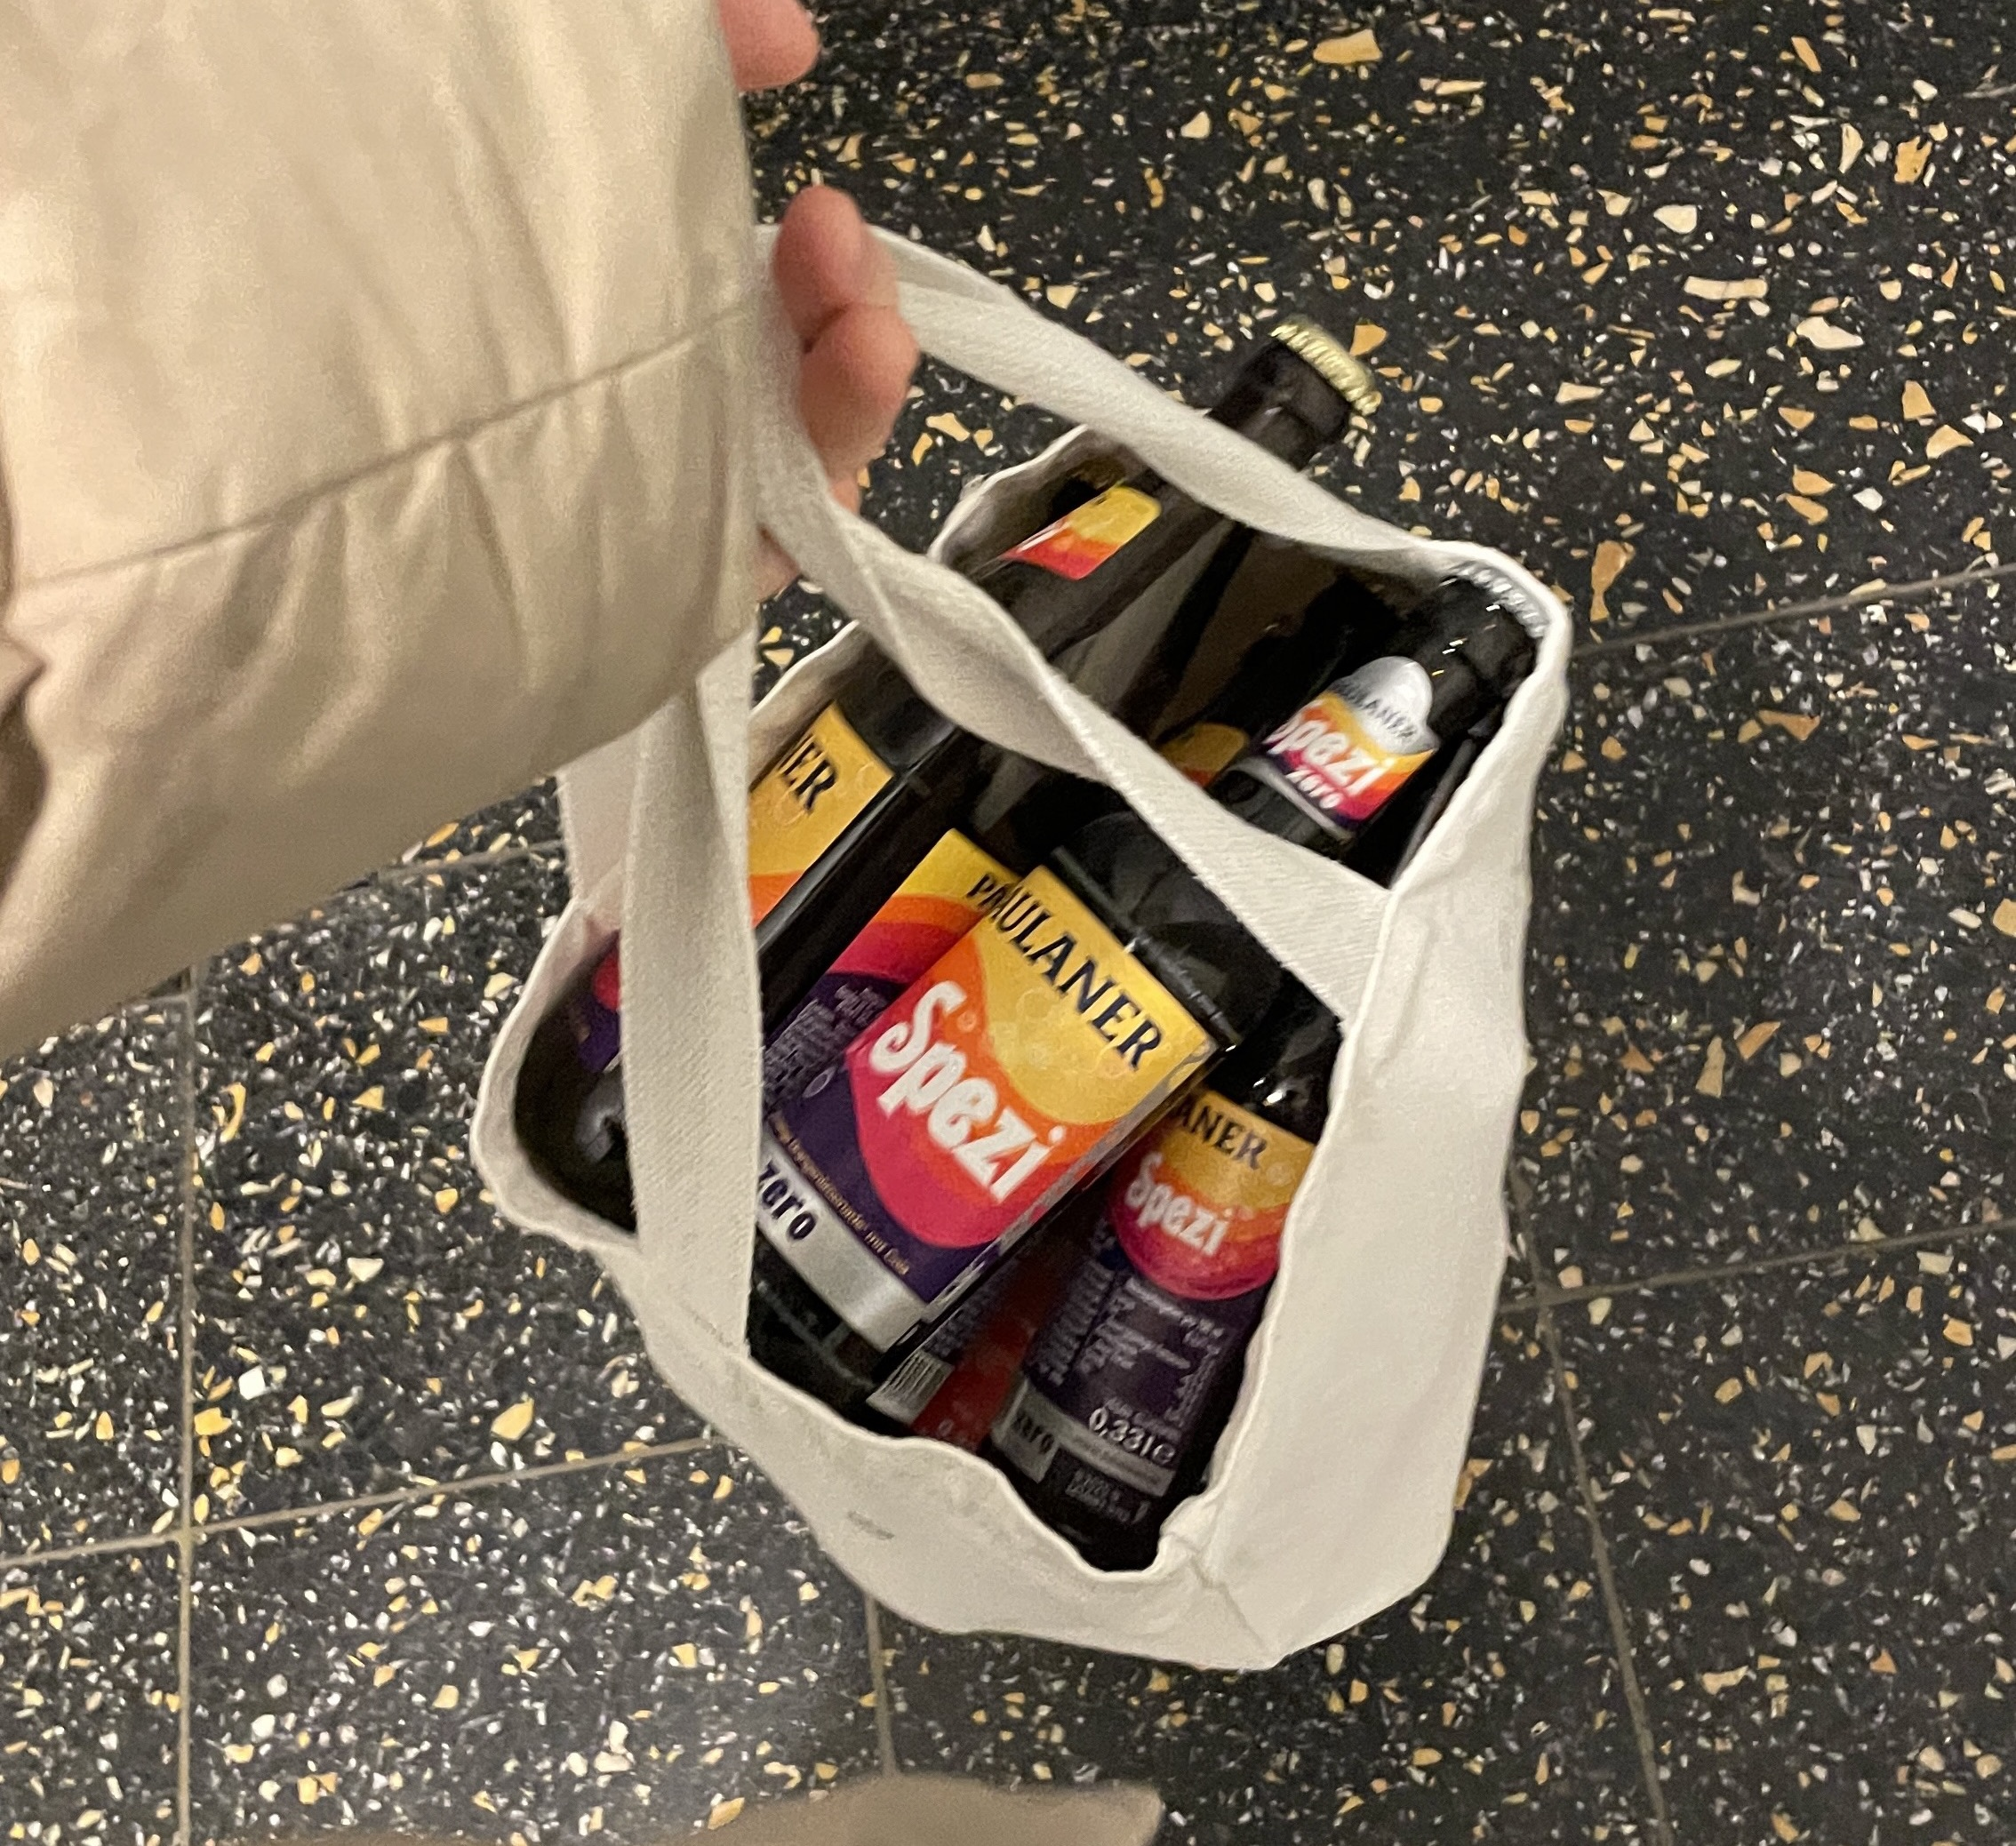
\includegraphics[width=.89\linewidth]
      {
        dummy_figure.JPG
      }%
      \label{fig:example:1}}
    \vfill
    \subfloat[My love Spezi.]{
      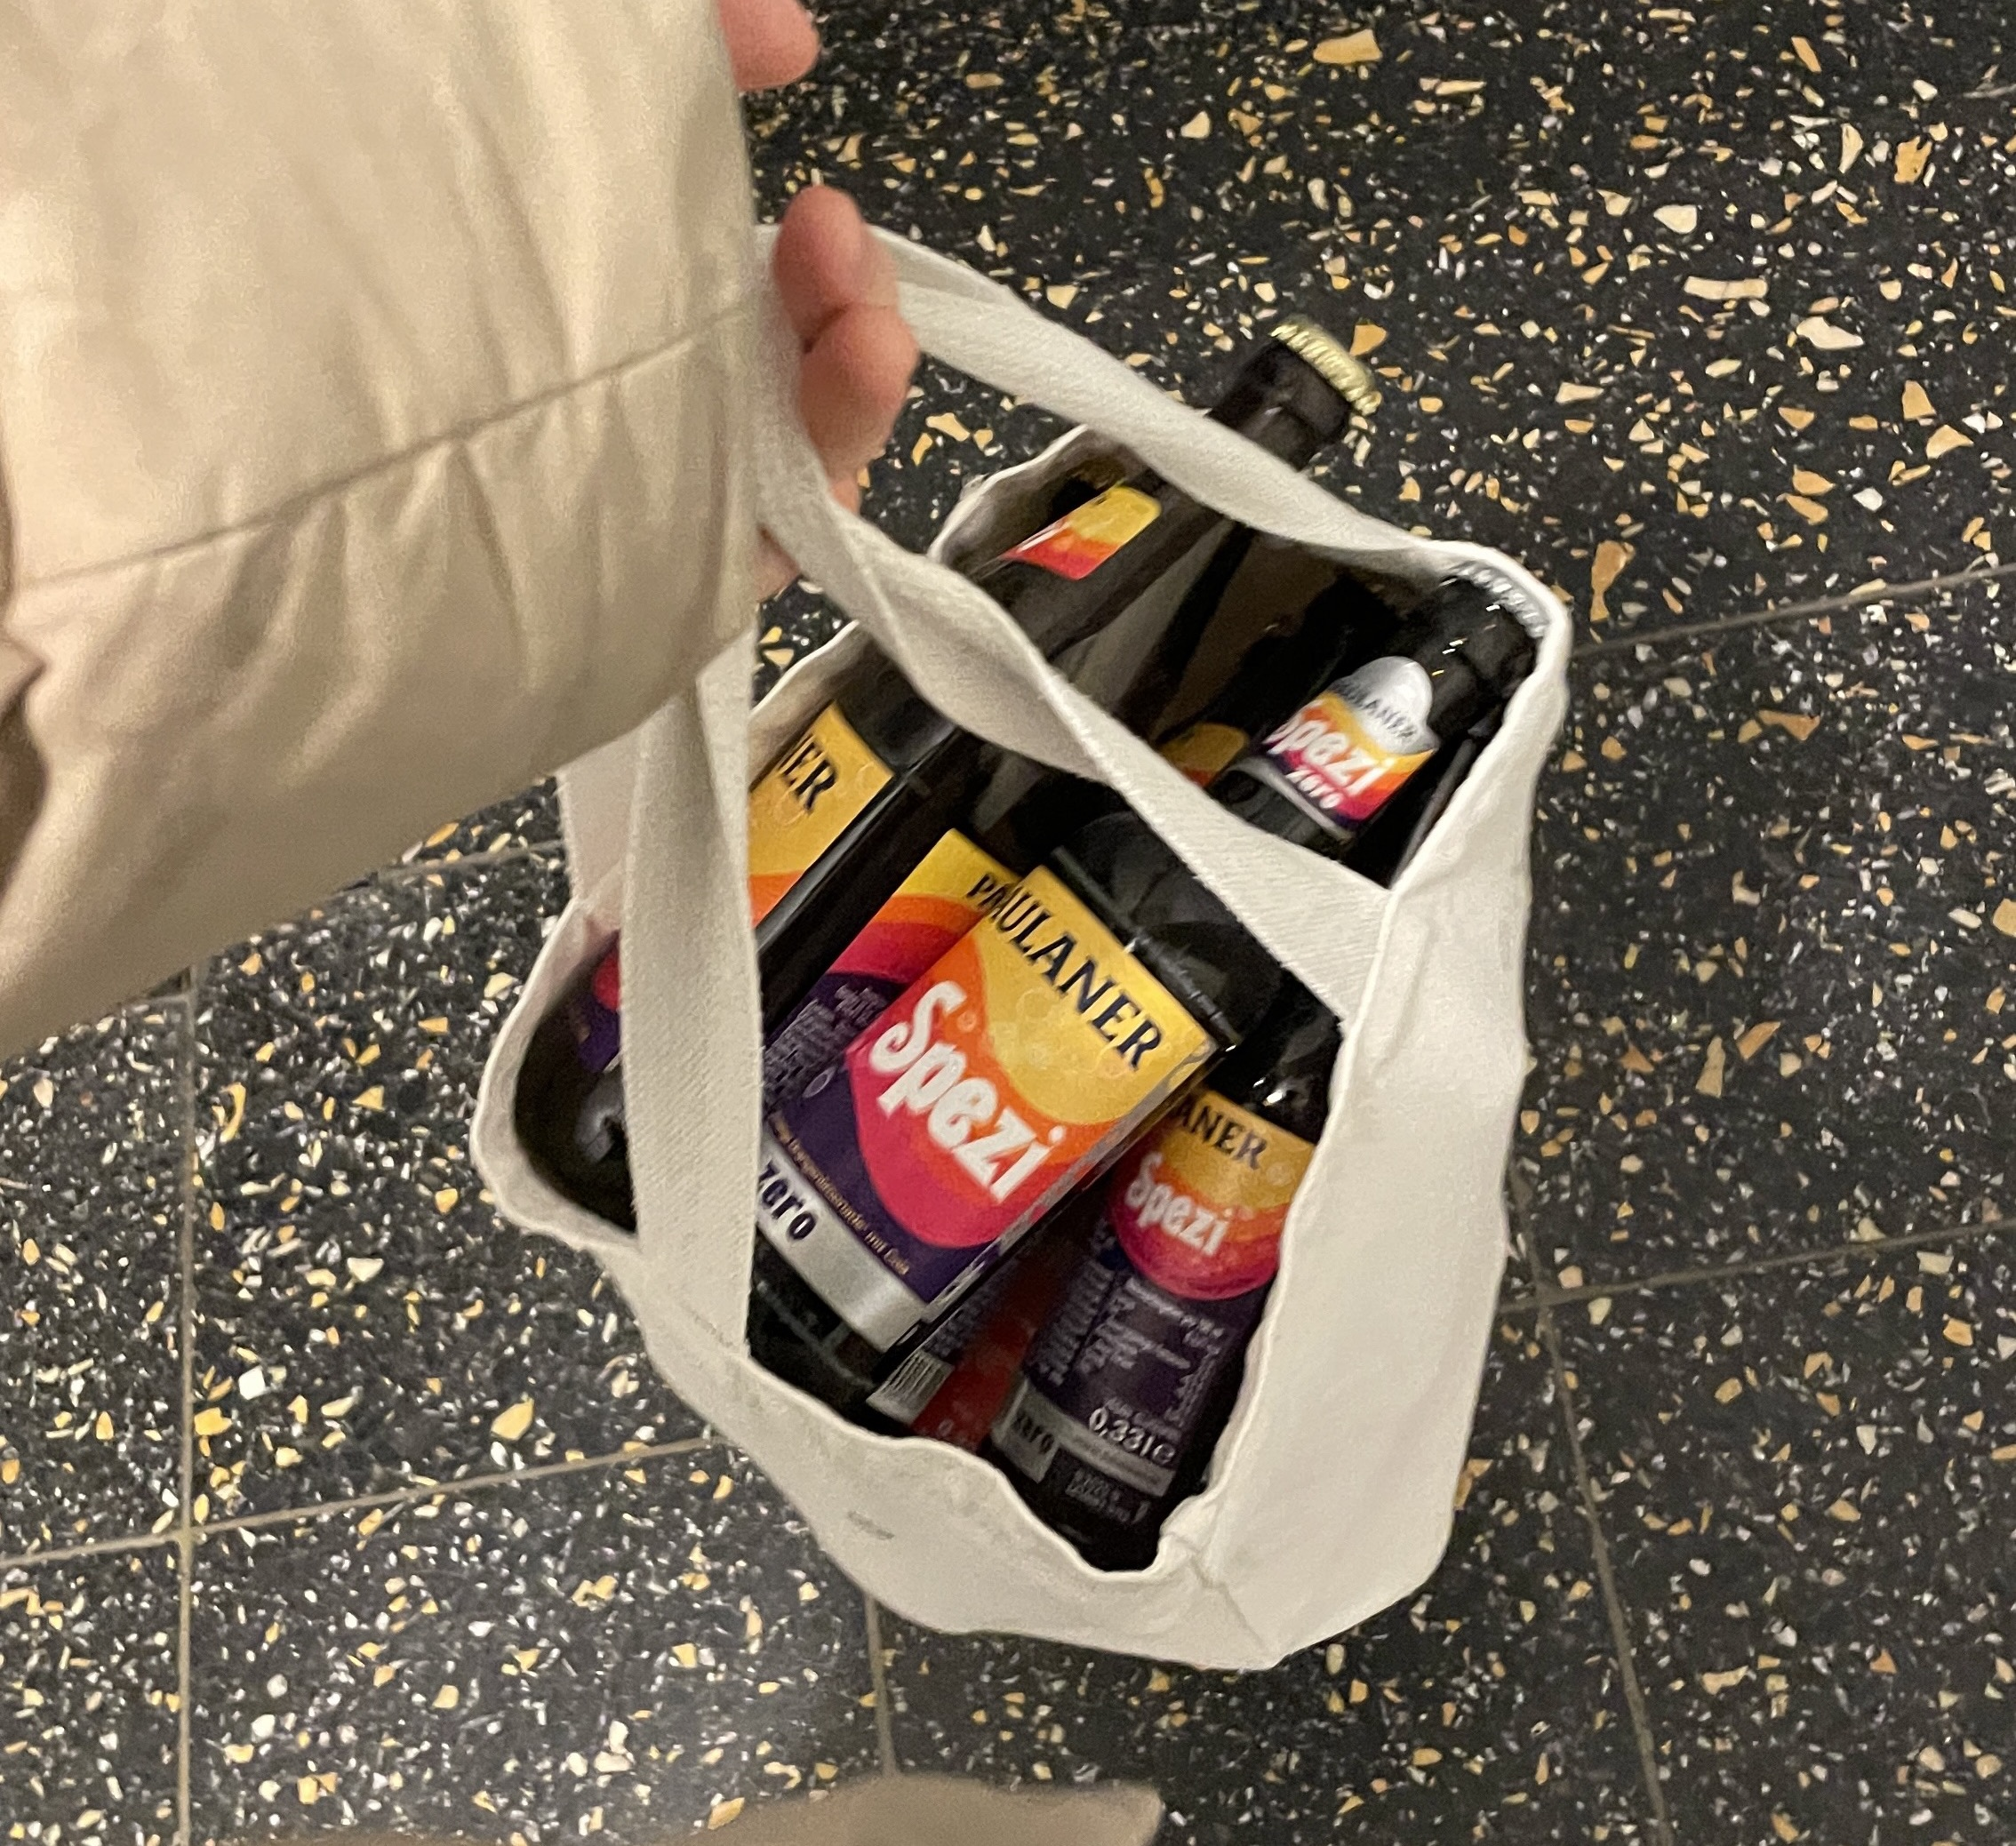
\includegraphics[width=.89\linewidth]
      {
        dummy_figure.JPG
      }%
      \label{fig:example:2}}      
    \caption{
    Example of subfigures.
    You can add colored lines like \protect\colorLine{blue}{solid} or \protect\colorLine{red}{dashed}, \ie you need to use $\protect$ in captions.
    By the way, the drinks in the figures are Spezi, which is my favorite drink in Munich, Germany.
  }
\label{fig:example}
\end{figure}

\begin{figure*}[t]
  \centering
    \subfloat[My love Spezi.]{
      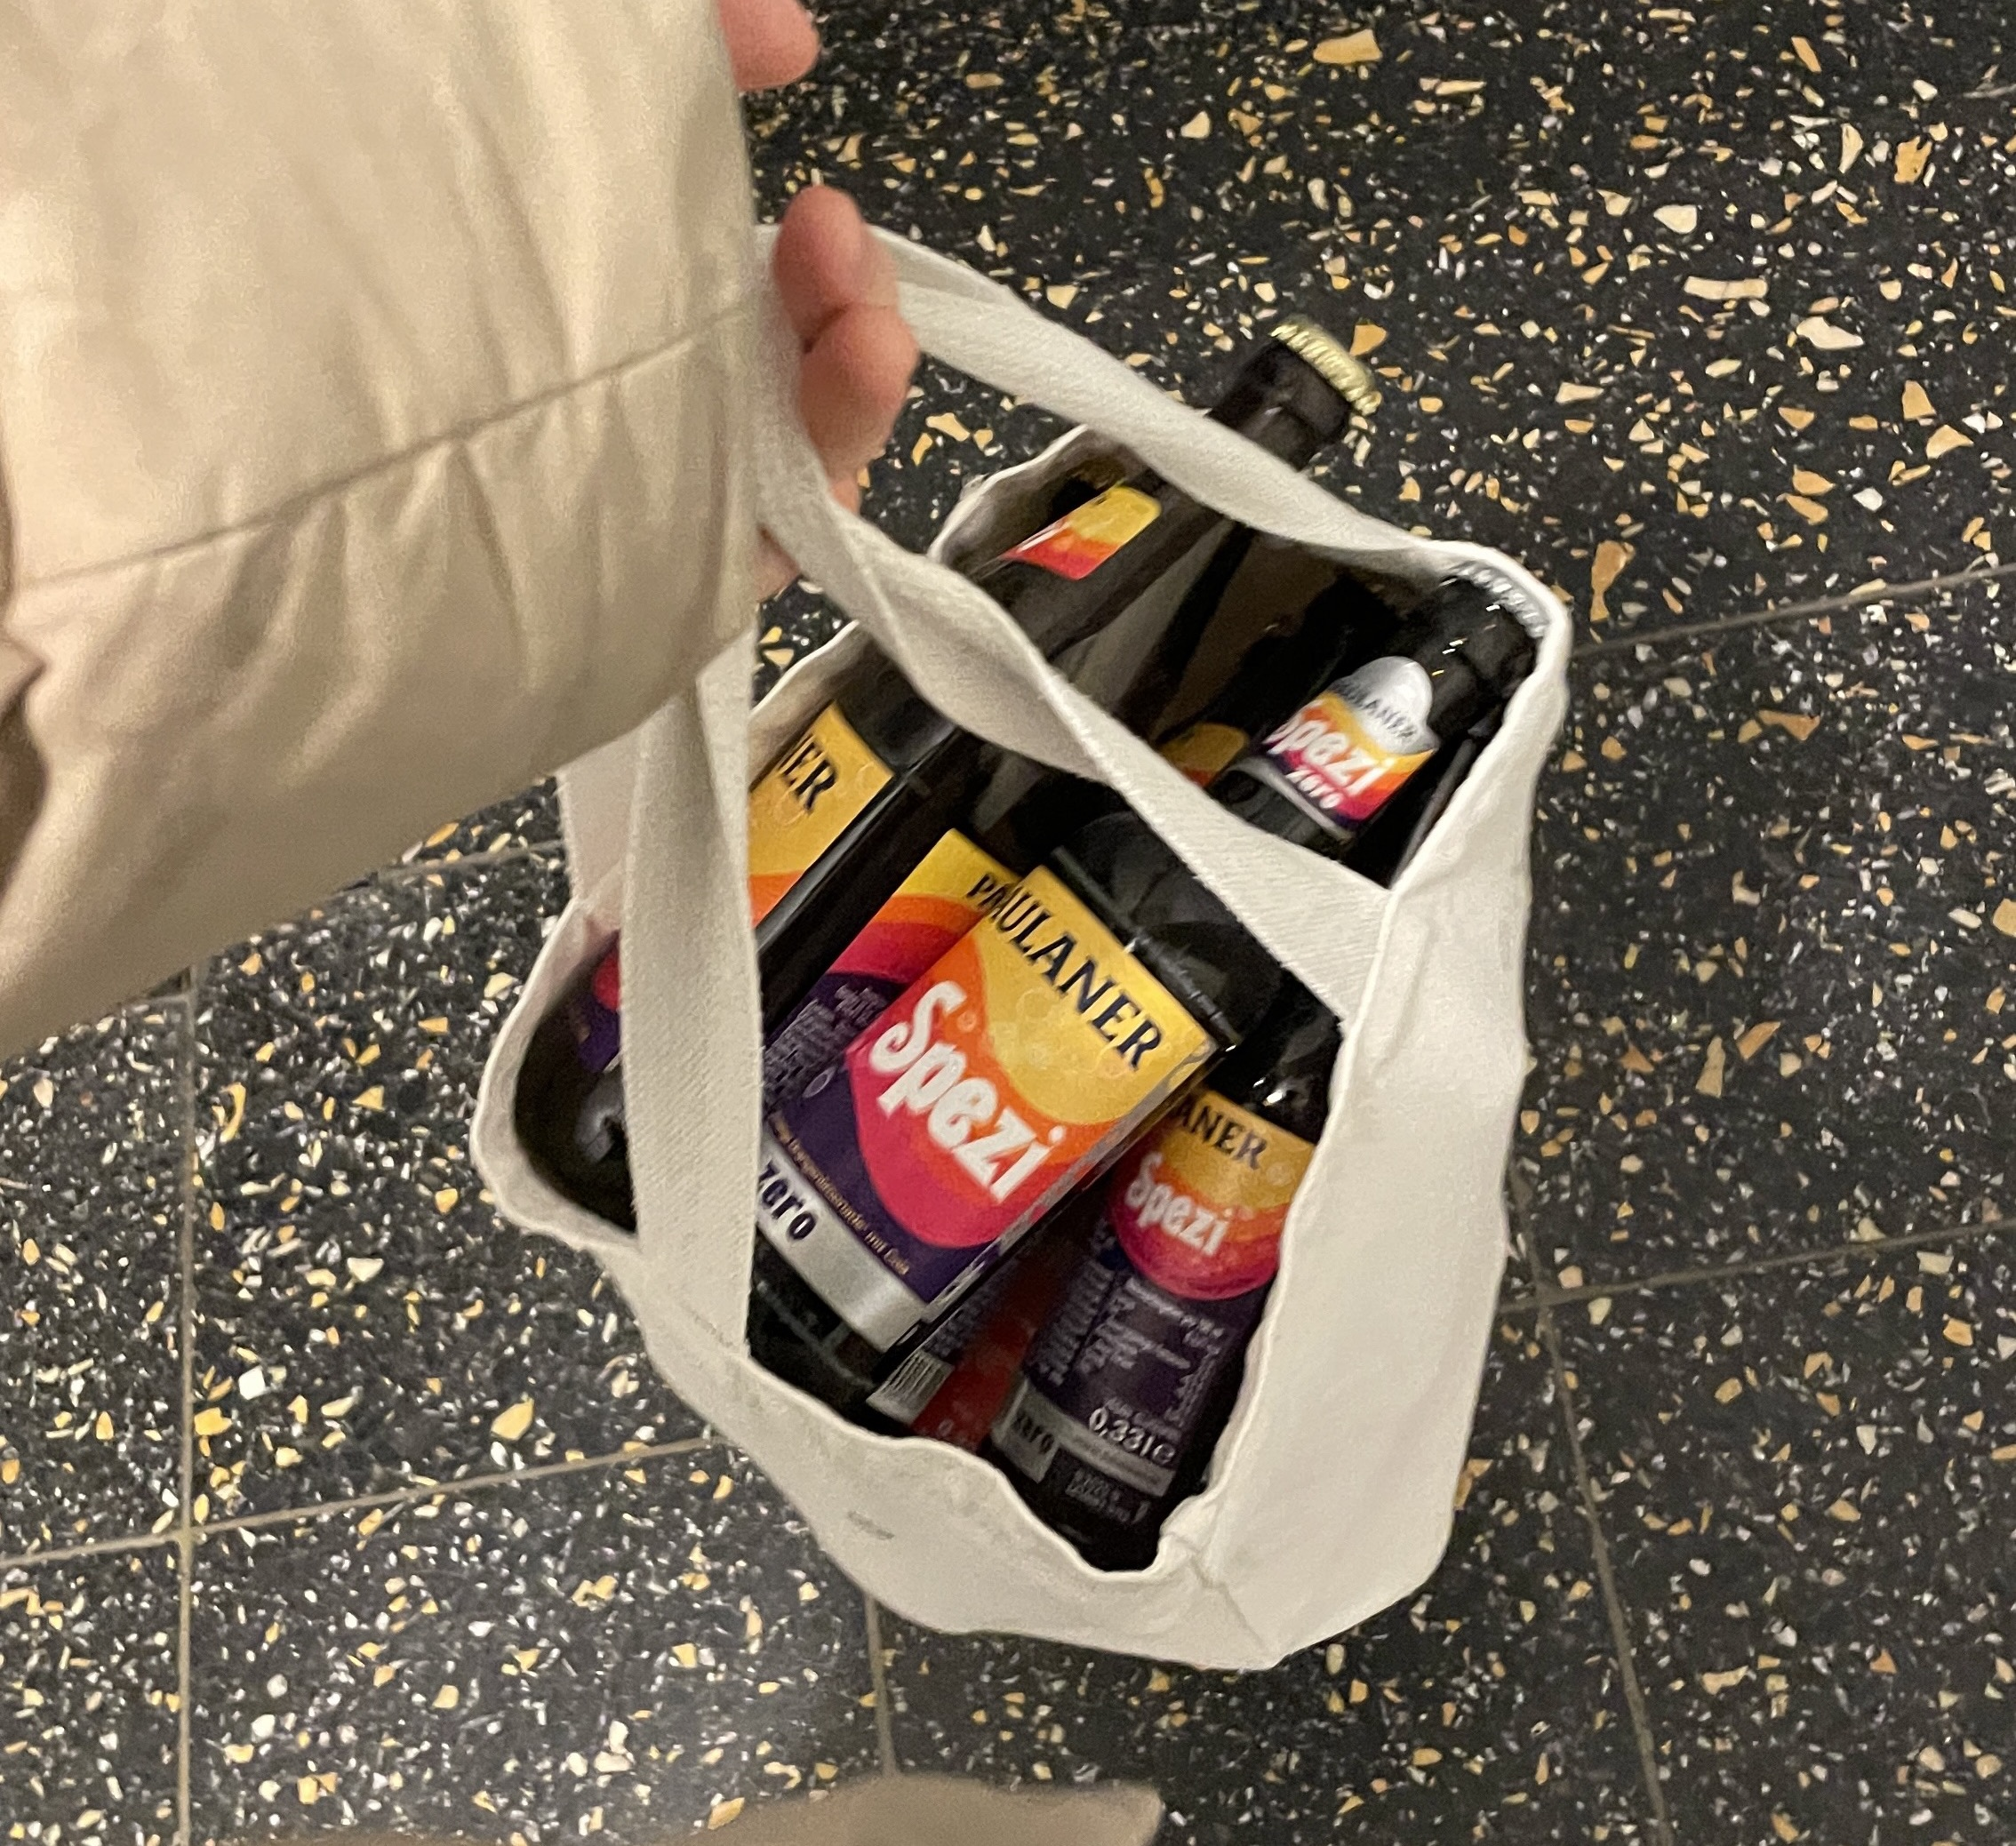
\includegraphics[width=.39\linewidth]
      {
        dummy_figure.JPG
      }%
      \label{fig:example:full:1}}
    \hfill
    \subfloat[My love Spezi.]{
      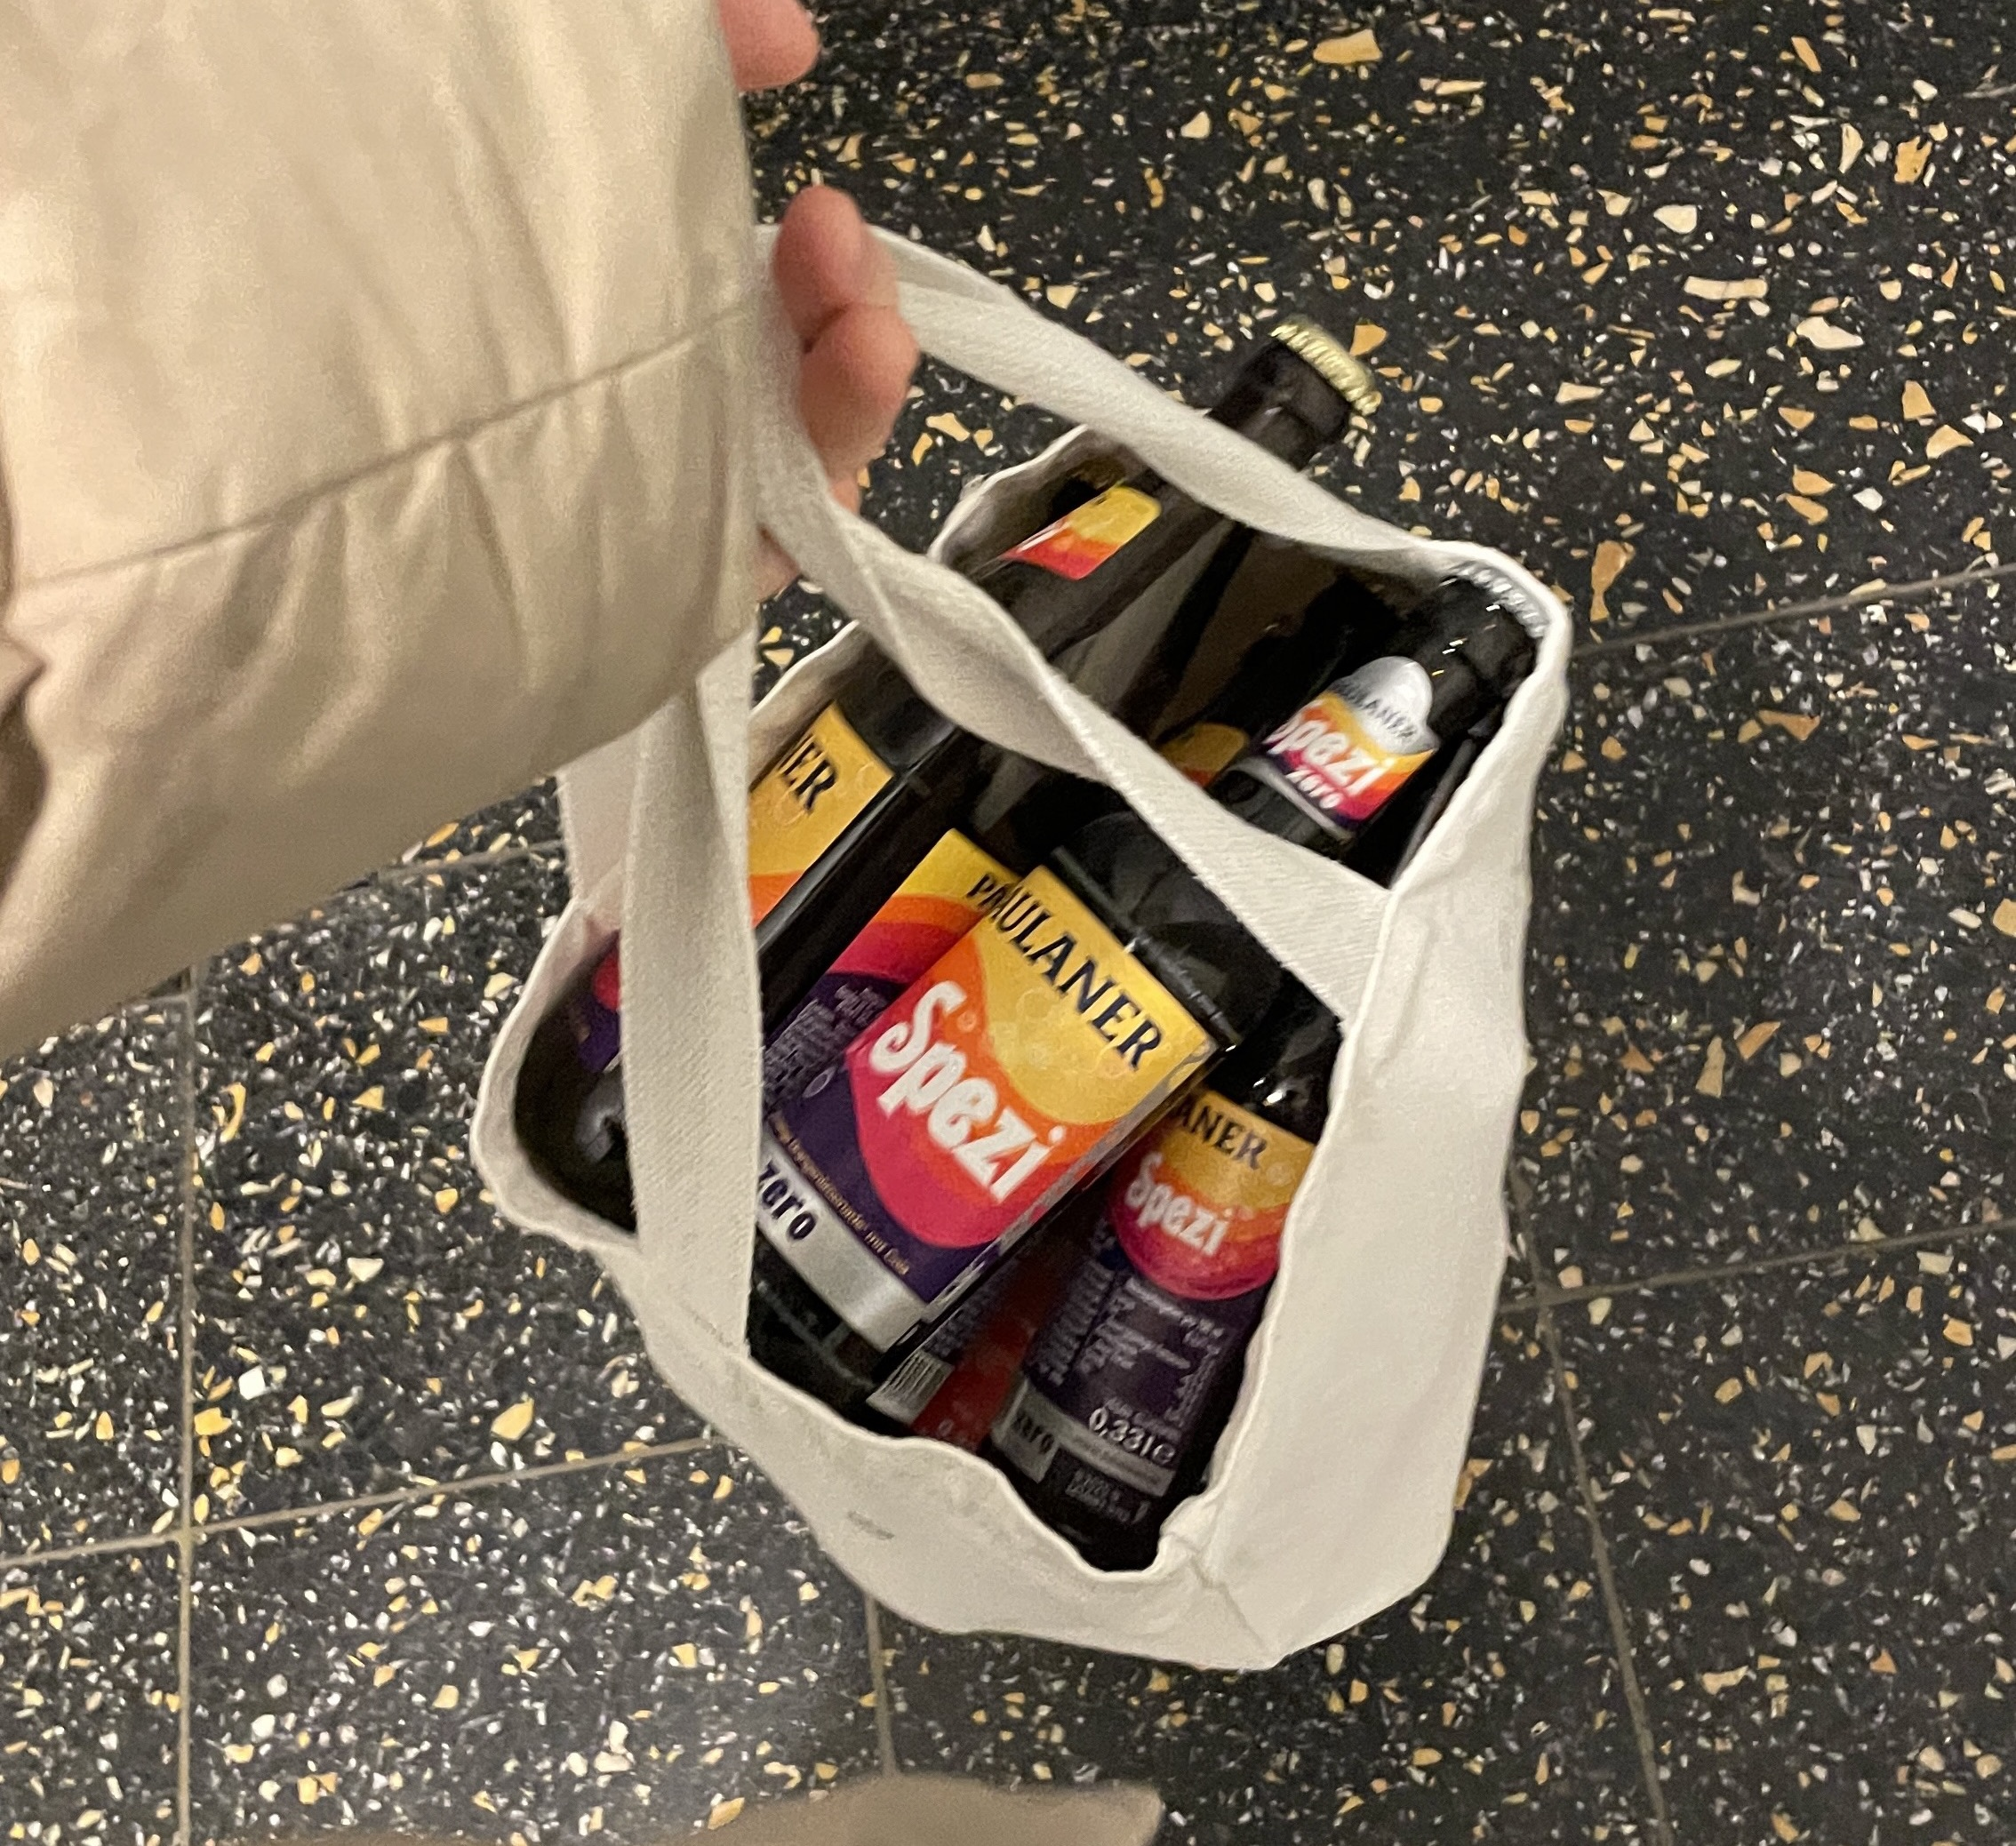
\includegraphics[width=.39\linewidth]
      {
        dummy_figure.JPG
      }%
      \label{fig:example:full:2}}      
    \caption{
    Example of subfigures in full width.
  }
\label{fig:example:full}
\end{figure*}

% ============================================
%                   Appendix
% ============================================
%% The Appendices part is started with the command \appendix;
%% appendix sections are then done as normal sections
\appendix

% ============================================
%                   Bibliography
% ============================================
\bibliographystyle{IEEEtran}
\bibliography{\template/refs}

% ============================================
%                   BIOGRAPHIES
% ============================================
\begin{IEEEbiography}[{
    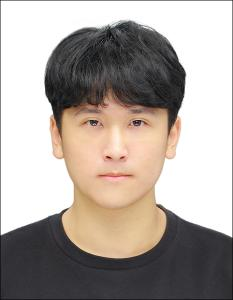
\includegraphics[width=1in,height=1.25in,clip,keepaspectratio]{\template/people/msRyu.jpg}}]{Myeongseok Ryu}
    received the B.S. degree in mechanical engineering from Incheon National University, South Korea, in 2023, and the M.S. degree in mechanical engineering from Gwangju Institute of Science and Technology (GIST), South Korea, in 2025. 
    He is currently serving as a researcher at the Cho Chun Shik Graduate School of Mobility, Korea Advanced Institute of Science and Technology (KAIST), South Korea.
    His research interests include adaptive control, neural-networks, and constrained optimization.
\end{IEEEbiography}

\begin{IEEEbiography}[{
    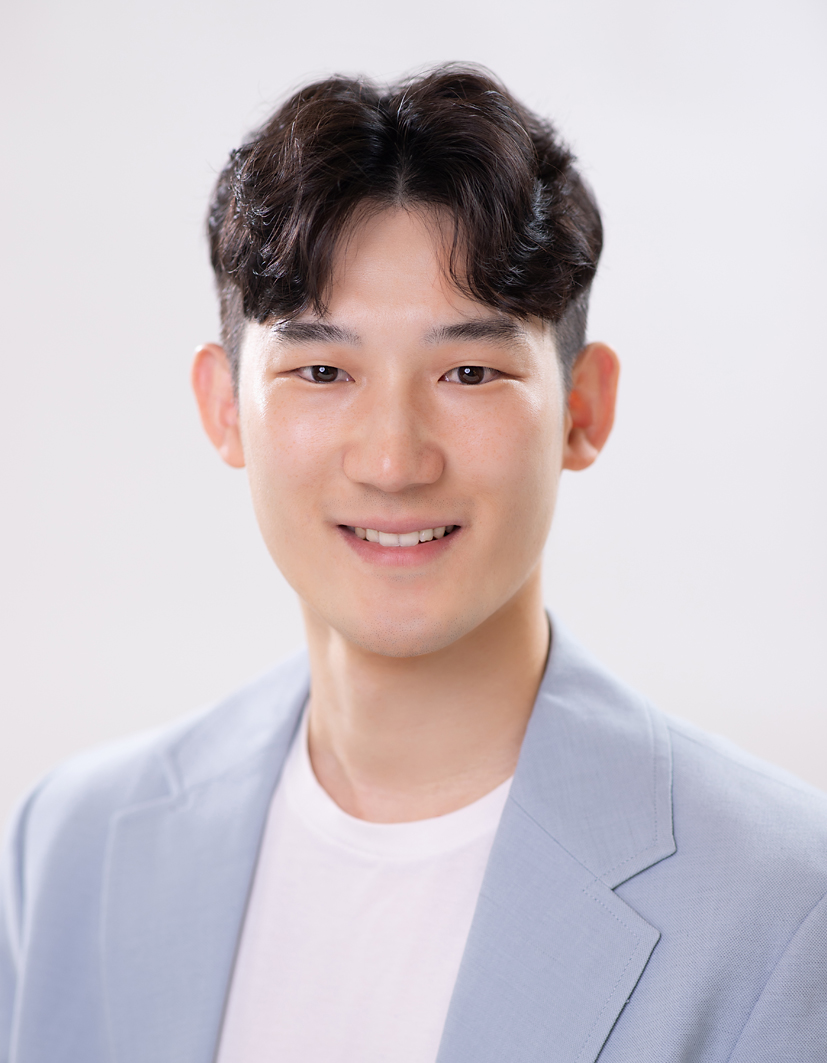
\includegraphics[width=1in,height=1.25in,clip,keepaspectratio]{\template/people/khChoi.jpg}}]{Kyunghwan Choi}
    Kyunghwan Choi received his B.S., M.S., and Ph.D. degrees in Mechanical Engineering from KAIST, Daejeon, South Korea, in 2014, 2016, and 2020, respectively. Following his Ph.D., he worked at the Center for Eco-Friendly \& Smart Vehicles at KAIST as a Postdoctoral Fellow and later as a Research Assistant Professor. In 2022, he joined GIST as an Assistant Professor in the Department of Mechanical and Robotics Engineering. Currently, he serves as an Assistant Professor at the Cho Chun Shik Graduate School of Mobility at KAIST, where he is also the Director of the Mobility Intelligence and Control Laboratory. His research focuses on optimal and learning-based control for connected, automated, and electrified vehicles (CAEVs).
\end{IEEEbiography}

\end{document}